\documentclass[t]{beamer}
\usepackage[utf8]{inputenc}
\usepackage[T1]{fontenc}
\usepackage{xcolor}
\usepackage{hyperref}
\title{Bayesian data analysis with TensorFlow Probability}
\date[ISPN ’80]{DataScienceConference Europe 2020}
\author{Simeon Carstens \& Dorran Howell, Tweag I/O}
\newcommand{\todo}{\textcolor{red}{\textbf{TODO}}}

%\usetheme{theme}

\begin{document}

\begin{frame}
  \titlepage
\end{frame}


\begin{frame}
  \frametitle{Your hosts}
  \begin{block}{Simeon}
    \raisebox{-0.5\height}{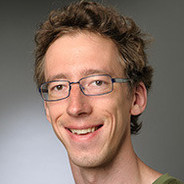
\includegraphics[width=0.15\paperwidth]{images/simeon}} ...will give the presentation \\
    \begin{itemize}
    \item background in computational structural biology
    \item Data Scientist at Tweag I/O since May 2019
    \end{itemize}
  \end{block}
  \begin{block}{Dorran}
    \raisebox{-0.5\height}{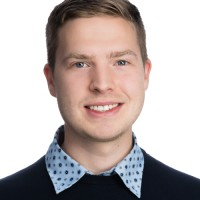
\includegraphics[width=0.15\paperwidth]{images/dorran}} ... will happily answers your questions in the chat\\
    \begin{itemize}
    \item background and previous positions in geophysics
    \item Data Scientist at Tweag I/O since August 2019
    \end{itemize}
  \end{block}
\end{frame}


\begin{frame}
  \frametitle{Tweag I/O}
  \todo \\
  Tweag I/O is a software innovation lab and consultancy based in Paris, but with employees all around the world.\\
  We specialize in
  \begin{itemize}
  \item software engineering, with a focus on functional programming
  \item DevOps, with a focus on reproducible software systems and builds
  \item data science
  \end{itemize}
\end{frame}


\begin{frame}
  \frametitle{What you're in for}
  This tutorial consists of alternating blocks of
  \begin{itemize}
  \item theory / example slides
  \item practical examples on either external websites or Google Colab notebooks. Links are provided at {\centering \url{https://github.com/tweag/tutorial-dsc-2020/}}
  \end{itemize}

  Requirements:
  \begin{itemize}
  \item a Google account (for the practical exercises)
  \item elementary knowledge in probability theory and statistics
  \end{itemize}
\end{frame}


\begin{frame}
  \frametitle{
\end{frame}


\end{document}